\documentclass[11pt]{article}
\usepackage{geometry} 
\geometry{a4paper,left=3cm,right=3cm, top=3cm, bottom=3cm}
\usepackage[parfill]{parskip}    % Activate to begin paragraphs with an empty line
\usepackage[T1]{fontenc}
\usepackage{graphicx}
\usepackage{tabularx}
\usepackage{fancyhdr}
\usepackage{lmodern}
\usepackage{amssymb}
\usepackage{epstopdf}
\usepackage{subfig}
\usepackage{hyperref}
\usepackage{mathtools}
\usepackage{listings}
\usepackage[table]{xcolor}

\newcommand{\groupNr}{49}
\newcommand{\assignmentNr}{3}

\pagestyle{fancy}
\fancyhf{}
\lfoot{SWA2011}
\cfoot{\thepage}
\rfoot{Group: \groupNr}
\renewcommand{\footrulewidth}{0.0pt}
\renewcommand{\headrulewidth}{0.0pt}

\begin{document}
{	
	\begin{figure}[h]
	\hspace{-1cm}
	
\includegraphics[height=23mm, width=170mm]{dsg-logo.png}
	\end{figure}

	\vspace{25mm}
	\centering
	{ \sffamily \Huge Assignment \assignmentNr } \\ \vspace{1mm}
	Software Architekturen \\ SS2010 \\ \vspace{10mm}
}

\noindent Group: \groupNr 
\begin{itemize}
\item Patrick Marschik, Mat. Nr.: 0625039, Stud. Kz.: 066 933 
\item Martin Schwengerer, Mat. Nr.: 0625209, Stud. Kz.: 066 937
\item Michael V\"ogler, Mat. Nr.: 0625617, Stud. Kz.: 066 937
\item Matthias Rauch, Mat. Nr.: 0626140, Stud. Kz.: 033 534
\item Benjamin Bachhuber, Mat. Nr.: 1028430, Stud. Kz.: 066 933 
\end{itemize}

\newpage
\tableofcontents

\newpage

\section{Technical Specification}

\begin{table}[h]
	\begin{tabularx}{\textwidth}{| X | X |}
	\hline
	\multicolumn{2}{|c|}{\textbf{Servers}} \\
	\hline
	\cellcolor[gray]{0.9}
	Application Server & Tomcat\\
	\hline
	\cellcolor[gray]{0.9}
	DBMS & PostgreSQL 8.4\\
	\hline
	\cellcolor[gray]{0.9}
	Cache & EhCache\\
	\hline
	\end{tabularx}
	\caption{Server technology}
	\label{server_tech}
\end{table}

\begin{table}[h]
	\begin{tabularx}{\textwidth}{| X | X |}
	\hline
	\multicolumn{2}{|c|}{\textbf{Frameworks}} \\
	\hline
	\cellcolor[gray]{0.9}
	Dependency Injection & Spring\\
	\hline
	\cellcolor[gray]{0.9}
	OR-Mapping & Hibernate\\
	\hline
	\cellcolor[gray]{0.9}
	Cache & EhCache\\
	\hline
	\cellcolor[gray]{0.9}
	MVC-Framework & Spring MVC \& J-Query\\
	\hline
	\cellcolor[gray]{0.9}
	Messaging & Spring Integration\\
	\hline
	\end{tabularx}
	\caption{Frameworks}
	\label{frameworks}
\end{table}


\begin{table}[h]
	\begin{tabularx}{\textwidth}{| X | X |}
	\hline
	\multicolumn{2}{|c|}{\textbf{Tools}} \\
	\hline
	\cellcolor[gray]{0.9}
	Build System & Maven\\
	\hline
	\cellcolor[gray]{0.9}
	IDE & IntelliJ\\
	\hline
	\cellcolor[gray]{0.9}
	Version Control System & Git\\
	\hline
	\end{tabularx}
	\caption{Tools}
	\label{tools}
\end{table}

\section{Prototype Architecture}

\subsection{(Entity) Class Diagram}

The class diagram (see Figure \ref{fig:class}) describes the basic domain model. The facts were assumed:

\begin{itemize}
\item The maps are created by the system and not the users.
\item Maps consist of tiles. Each tile can have a base which consists of 32 squares
\item Upgrading buildings and sending troops takes some time
\item Creating troops and running buildings may cost some resources.
\end{itemize}

The User embeds adddress information and stores the difference to UTC to ensure messages are sent in right order. All other dates are stored in UTC. Troop and TroopGroup uses the Composite Object Pattern. A Building can either be a ResourceBuilding (for mining resources) or a NormalBuilding. Every Action performed by a certain user is stored in the database.

\subsection{Component Diagram}

The component diagram (see Figure \ref{fig:component}) illustrates the interaction between the components. The web  interface is the only component located in the presentation layer. The Map Controller is the core component and offers interfaces for browsing, troop management, building management and resource management. Itself depends on Persistence and the Notification Controller. The User Management Component offers interfaces for registration/deletion of accounts and session management. The Statistics component offers functionality about the ranking of players and so on. Finally the Storage component is used to store and retrieve data from the database. The Cache component offers the same interface as the Storage component, since it should be transparent for the client wether or not caching is enabled.

\subsection{Deployment Diagram}

Text \dots (see Figure \ref{fig:deployment}) \dots Text \dots

\subsubsection{Uptime Calculation}

The deployment diagram shows three main sites where artifacts have to be deployed. 
\begin{enumerate}
\item There exists a cluster hosting Map Controller and the corresponding database for each map in the game. The cluster itself can be divided into several nodes that can server requests for this map. A load balancer is responsible for the request routing. The databases of the nodes must be replicated since they hold the same set of data.
\item A similar cluster hosting the User Management component serves registration and session management requests.
\item Another cluster is responsible for processing messaging requests. As denoted in D-1 there exists a message queue for each node of the cluster to provide reliable messaging. A redundant network of SMTP servers ensures availability of e-mail notifications.
\end{enumerate}

This redundancy of services is necessary on the one hand to fulfill the performance requirements and provide a scalable architecture. On the other hand it results in a fail safe system as the following calculation shows:

\begin{itemize}
\item $P(nodeFails) = 0.1$
\end{itemize}

As the requirements specification denotes we can assume that each node has a failure probability of $10\%$.

A cluster consists of n nodes. Since the cluster is available when at least one node is available we can set failure possibility of a cluster.

\begin{itemize}
\item $P(clusterFails) = 0.1^n$
\end{itemize}

When we consider that we have three cluster in our system, we get the formula for the overall system fail rate:

\begin{itemize}
\item $P(clusterFails) = 3 *0.1^n$
\end{itemize}

To calculate availability we have to consider the inverse probability:

\begin{itemize}
\item $P(systemAvailable) = 1 - 3 *0.1^n$
\end{itemize}

If we solve the inequality

\begin{itemize}
\item $1 - 3 *0.1^n \ge 0.99999$
\end{itemize}

we receive

\begin{itemize}
\item $n \ge 4.47712 \implies n \ge 5$
\end{itemize}

That means if that we reach an availability of $99,99\%$ if we have at least 5 nodes in each cluster. To fulfill security requirements the communication between server and client is always encrypted.

\newpage

\subsection{Architectural Decisions}

\subsubsection{D-1}

\begin{table}[h] \small
	\begin{tabularx}{\textwidth}{ | l | X |}
    	\hline
	\cellcolor[gray]{0.9}
    	\textbf{Issue} & There can be lots of simultaneous messages and not all of them can be handled by the database and mail servers directly. \\
	\hline
	\cellcolor[gray]{0.9}
	\textbf{Decision} & Use an asynchronous message queue as buffer for sent messages. The middleware has to offer a queue for each Notification node. \\ 
	\hline
	\cellcolor[gray]{0.9}
	\textbf{Group} & Component Interaction \\ 
	\hline
	\cellcolor[gray]{0.9}
	\textbf{Assumptions} & 
		\begin{itemize}
		\item Lots of simultaneous messages
		\item Not all of them can be handled directly by processing nodes 
		\end{itemize} \\ 
	\hline
	\cellcolor[gray]{0.9}
	\textbf{Constraints} & - \\ 
	\hline
	\cellcolor[gray]{0.9}
	\textbf{Positions} &  
		\begin{itemize}
		\item Directly send/store messages at the mail server resp. database server using explicit invocation.
		\item Use one single message queue for all e-mails and use one single for all internal messages.
		\end{itemize} \\ 	
	\hline
	\cellcolor[gray]{0.9}
	\textbf{Argument} & Message queues buffer messages to ensure the system can cope with load peeks. Since processing of the message is delayed a call to the Notification Component would take a much smaller amount of time. I also decided to use a queue for each processing node, since a central queue would cause a single-point of failure. \\ 
	\hline
	\cellcolor[gray]{0.9}
	\textbf{Implications} & The middleware must be chosen appropriately to support asynchronous message queues. \\ 
	\hline
	\cellcolor[gray]{0.9}
	\textbf{Related decisions} & - \\ 
	\hline
	\cellcolor[gray]{0.9}
	\textbf{Related requirements} & 
		\begin{itemize}
		\item There can be lots of simultaneous messages and not all of them can be handled by the database and mail servers directly.
		\item Make sure that notifications are reliable and do not simply rely on the database or, even worse, the mail server.
		\end{itemize}\\
	\hline
	\cellcolor[gray]{0.9}
	\textbf{Related artifacts} & requirements specification, component diagram, deployment diagram \\
	\hline
	\cellcolor[gray]{0.9}
	\textbf{Related principles} & -\\
	\hline
	\end{tabularx}
	\caption{Design decision - D-1}
	\label{dec:D1}
\end{table}

\newpage

\subsubsection{D-2}

\begin{table}[h] \small
	\begin{tabularx}{\textwidth}{ | l | X |}
    	\hline
	\cellcolor[gray]{0.9}
    	\textbf{Issue} & A complex system should be divided into components to enforce separation of concerns and provide reusability and modifiability. \\
	\hline
	\cellcolor[gray]{0.9}
	\textbf{Decision} & Structure the architecture into layers, s.t. higher layers depend on lower layers. \\ 
	\hline
	\cellcolor[gray]{0.9}
	\textbf{Group} & Component Interaction \\ 
	\hline
	\cellcolor[gray]{0.9}
	\textbf{Assumptions} & 
		\begin{itemize}
		\item The functionality can be grouped into components.
		\item The components can define interfaces to make their functionality externally available.
		\end{itemize}\\ 
	\hline
	\cellcolor[gray]{0.9}
	\textbf{Constraints} & - \\ 
	\hline
	\cellcolor[gray]{0.9}
	\textbf{Positions} & 
		\begin{itemize}
		\item Use strong coupling between components.
		\item Use a monolithic design.
		\end{itemize}\\ 
	\hline
	\cellcolor[gray]{0.9}
	\textbf{Argument} & Some low-level parts of the system (e.g. Persistence, Access Control) are used by many higher-level parts. Strong coupling between components would restrain us concerning modifications be done in future, since we could not exchange components. A monolithic design on the other hand restrains concerning distributability of the components. \\ 
	\hline
	\cellcolor[gray]{0.9}
	\textbf{Implications} & The architecture should be grouped into the following layers (from high to low):
		\begin{enumerate}
		\item Presentation
		\item Business Logic (Maps, Statistics, User Management)
		\item Access Control
		\item Cache
		\item Persistence 
		\end{enumerate}\\ 
	\hline
	\cellcolor[gray]{0.9}
	\textbf{Related decisions} & - \\ 
	\hline
	\cellcolor[gray]{0.9}
	\textbf{Related requirements} & -\\
	\hline
	\cellcolor[gray]{0.9}
	\textbf{Related artifacts} & Component diagram\\
	\hline
	\cellcolor[gray]{0.9}
	\textbf{Related principles} & Dependency Injection\\
	\hline
	\end{tabularx}
	\caption{Design decision - D-2}
	\label{dec:D2}
\end{table}

\newpage

\subsubsection{D-3}

\begin{table}[h] \small
	\begin{tabularx}{\textwidth}{ | l | X |}
    	\hline
	\cellcolor[gray]{0.9}
    	\textbf{Issue} & Important actions have to be logged. It is also necessary to monitor system performance. \\
	\hline
	\cellcolor[gray]{0.9}
	\textbf{Decision} & Use the Interceptor pattern. \\ 
	\hline
	\cellcolor[gray]{0.9}
	\textbf{Group} & Adaption \\ 
	\hline
	\cellcolor[gray]{0.9}
	\textbf{Assumptions} & There exist well-defined points where interceptors can be plugged in. \\ 
	\hline
	\cellcolor[gray]{0.9}
	\textbf{Constraints} & - \\ 
	\hline
	\cellcolor[gray]{0.9}
	\textbf{Positions} & 
		\begin{itemize}
		\item Use hard-coded logging in each component.
		\item Use profiling tools to monitor application and database.
		\end{itemize}\\ 
	\hline
	\cellcolor[gray]{0.9}
	\textbf{Argument} & The interceptor pattern provides hooks, where additional functionality can be injected. Thus not only auditing is supported. In contrast to hard-coded logging, interceptors can also be injected at run-time, if the configuration supports it. Compared to profiling tools, interceptors support all execution environments and databases. Besides that profiling tools consume more resources. \\ 
	\hline
	\cellcolor[gray]{0.9}
	\textbf{Implications} & Interceptors should be pluggable in the following scenarios:
		\begin{itemize}
		\item user login/logout
		\item action start/end
		\item database access
		\item notification sending/receiving
		\item complex calculations (map generation, attacks, etc.) 
		\end{itemize}\\ 
	\hline
	\cellcolor[gray]{0.9}
	\textbf{Related decisions} & - \\ 
	\hline
	\cellcolor[gray]{0.9}
	\textbf{Related requirements} & Every important action in the system has to be logged. There should be a user ranking which can be seen by every user: user with most points, richest user, strongest troop type, and so on. Also try to monitor some aspects of the system performance (e.g., average processing times, resource usage) and the system configuration itself (e.g., currently active nodes). Try to keep this information as up-to-date as possible, but do not create it directly from live data.\\
	\hline
	\cellcolor[gray]{0.9}
	\textbf{Related artifacts} & Requirements specification\\
	\hline
	\cellcolor[gray]{0.9}
	\textbf{Related principles} & -\\
	\hline
	\end{tabularx}
	\caption{Design decision - D-3}
	\label{dec:D3}
\end{table}

\newpage

\subsubsection{D-4}

\begin{table}[h] \small
	\begin{tabularx}{\textwidth}{ | l | X |}
    	\hline
	\cellcolor[gray]{0.9}
    	\textbf{Issue} & No other user should be able to access or manipulate sensitive data of other users. \\
	\hline
	\cellcolor[gray]{0.9}
	\textbf{Decision} & Provide special interceptors to ensure access control. \\ 
	\hline
	\cellcolor[gray]{0.9}
	\textbf{Group} & Adaptation \\ 
	\hline
	\cellcolor[gray]{0.9}
	\textbf{Assumptions} & The system supports interceptors. \\ 
	\hline
	\cellcolor[gray]{0.9}
	\textbf{Constraints} & - \\ 
	\hline
	\cellcolor[gray]{0.9}
	\textbf{Positions} & 
		\begin{itemize}
		\item Implement access control in database.
		\item Implement access control directly in the business logic.
		\end{itemize}\\ 
	\hline
	\cellcolor[gray]{0.9}
	\textbf{Argument} & Realizing access control via interceptors has two advantages compared with the other positions: Firstly as denoted in D-3 interceptors can be plugged into the system at run-time. This means changes in access control don't demand the rollout of a new version and therefore do not result in downtime. Secondly the business code isn't messed up with security specific code and therefore easier to read, which directly corresponds to better maintainability and a lower bug rate. \\ 
	\hline
	\cellcolor[gray]{0.9}
	\textbf{Implications} & Security interceptors should be placed at the following scenarios:
		\begin{itemize}
		\item action start
		\item database access
		\end{itemize}\\ 
	\hline
	\cellcolor[gray]{0.9}
	\textbf{Related decisions} & D-3 \\ 
	\hline
	\cellcolor[gray]{0.9}
	\textbf{Related requirements} & The system has strong security requirements, and you should prevent users from cheating or manipulating the game. No other user should be able to access or manipulate sensitive data of other users.\\
	\hline
	\cellcolor[gray]{0.9}
	\textbf{Related artifacts} & Requirements specification\\
	\hline
	\cellcolor[gray]{0.9}
	\textbf{Related principles} & -\\
	\hline
	\end{tabularx}
	\caption{Design decision - D-4}
	\label{dec:D4}
\end{table}

\newpage

\subsubsection{D-5}

\begin{table}[h] \small
	\begin{tabularx}{\textwidth}{ | l | X |}
    	\hline
	\cellcolor[gray]{0.9}
    	\textbf{Issue} & Performance is crucial. The system needs to handle 1000's of concurrent users. \\
	\hline
	\cellcolor[gray]{0.9}
	\textbf{Decision} & It should be possible to partition the system horizontally for each map. That means that each map should have a denoted server (or server farm). Besides that each node has a cache to minimize database roundtrips. \\ 
	\hline
	\cellcolor[gray]{0.9}
	\textbf{Group} & Performance \\ 
	\hline
	\cellcolor[gray]{0.9}
	\textbf{Assumptions} & The system can be partitioned horizontally for each map. \\ 
	\hline
	\cellcolor[gray]{0.9}
	\textbf{Constraints} & - \\ 
	\hline
	\cellcolor[gray]{0.9}
	\textbf{Positions} & 
		\begin{itemize}
		\item Set up a single server that is strong enough to handle 1000's of users.
		\item Set up many nodes that mirror the whole database.
		\end{itemize}\\ 
	\hline
	\cellcolor[gray]{0.9}
	\textbf{Argument} & Distributing the application logic over more than one server is a good idea for scenarios where performance and availability are key requirements. Concerning availability clustering has the benefit that we don't have a single point of failure. Besides that in our concrete scenario, the map is the perfect choice for a partition criteria, since there are no cross-map operations possible by requirements specification. This results in less replication overhead. \\ 
	\hline
	\cellcolor[gray]{0.9}
	\textbf{Implications} & Load balancing \\ 
	\hline
	\cellcolor[gray]{0.9}
	\textbf{Related decisions} & D-2 (cache layer) \\ 
	\hline
	\cellcolor[gray]{0.9}
	\textbf{Related requirements} & Performance must be consistent. It is not acceptable for a user to have to wait more than two or three seconds when submitting a post or loading a page. So think about a good strategy how to scale all parts of the application.\\
	\hline
	\cellcolor[gray]{0.9}
	\textbf{Related artifacts} & Requirements specification, deployment diagram\\
	\hline
	\cellcolor[gray]{0.9}
	\textbf{Related principles} & -\\
	\hline
	\end{tabularx}
	\caption{Design decision - D-5}
	\label{dec:D5}
\end{table}

\newpage

\subsubsection{D-1}

\begin{table}[h] \small
	\begin{tabularx}{\textwidth}{ | l | X |}
    	\hline
	\cellcolor[gray]{0.9}
    	\textbf{Issue} & TODO \\
	\hline
	\cellcolor[gray]{0.9}
	\textbf{Decision} & TODO \\ 
	\hline
	\cellcolor[gray]{0.9}
	\textbf{Group} & TODO \\ 
	\hline
	\cellcolor[gray]{0.9}
	\textbf{Assumptions} & TODO \\ 
	\hline
	\cellcolor[gray]{0.9}
	\textbf{Constraints} & TODO \\ 
	\hline
	\cellcolor[gray]{0.9}
	\textbf{Positions} & TODO \\ 
	\hline
	\cellcolor[gray]{0.9}
	\textbf{Argument} & TODO \\ 
	\hline
	\cellcolor[gray]{0.9}
	\textbf{Implications} & TODO \\ 
	\hline
	\cellcolor[gray]{0.9}
	\textbf{Related decisions} & TODO \\ 
	\hline
	\cellcolor[gray]{0.9}
	\textbf{Related requirements} & TODO\\
	\hline
	\cellcolor[gray]{0.9}
	\textbf{Related artifacts} & TODO\\
	\hline
	\cellcolor[gray]{0.9}
	\textbf{Related principles} & TODO\\
	\hline
	\end{tabularx}
	\caption{Design decision - D-1}
	\label{dec:D1}
\end{table}

\subsection{Future work}

\begin{itemize}
\item Load-Balancer?
\item https?
\end{itemize}

\section{Prototype Installation Guidelines}

\subsection{Requirements}

\begin{itemize}
\item Tomcat 6 or 7 running on \texttt{localhost:8080/}
\item PostgreSQL 8.4 running on \texttt{localhost:5432/}
	\begin{itemize}
	\item Database: \texttt{swa}
		\begin{itemize}
		\item accessible by user: \texttt{swa}
		\item password for user: \texttt{swa11}
		\end{itemize}
	\end{itemize}
\item Ant or Maven
\end{itemize}

Run quartz script!!

\subsection{Compiling and Deploying}

\subsection{Entry Point}

The entry point to play \textbf{SWAG} is \href{http:localhost:8080/user/swag/user/}{http:localhost:8080/user/swag/user/}. There you can register an user, login and choose a map to play on.

\newpage

\pagenumbering{Roman}
\appendix
\section{Figures}

\begin{figure}[h]
\center
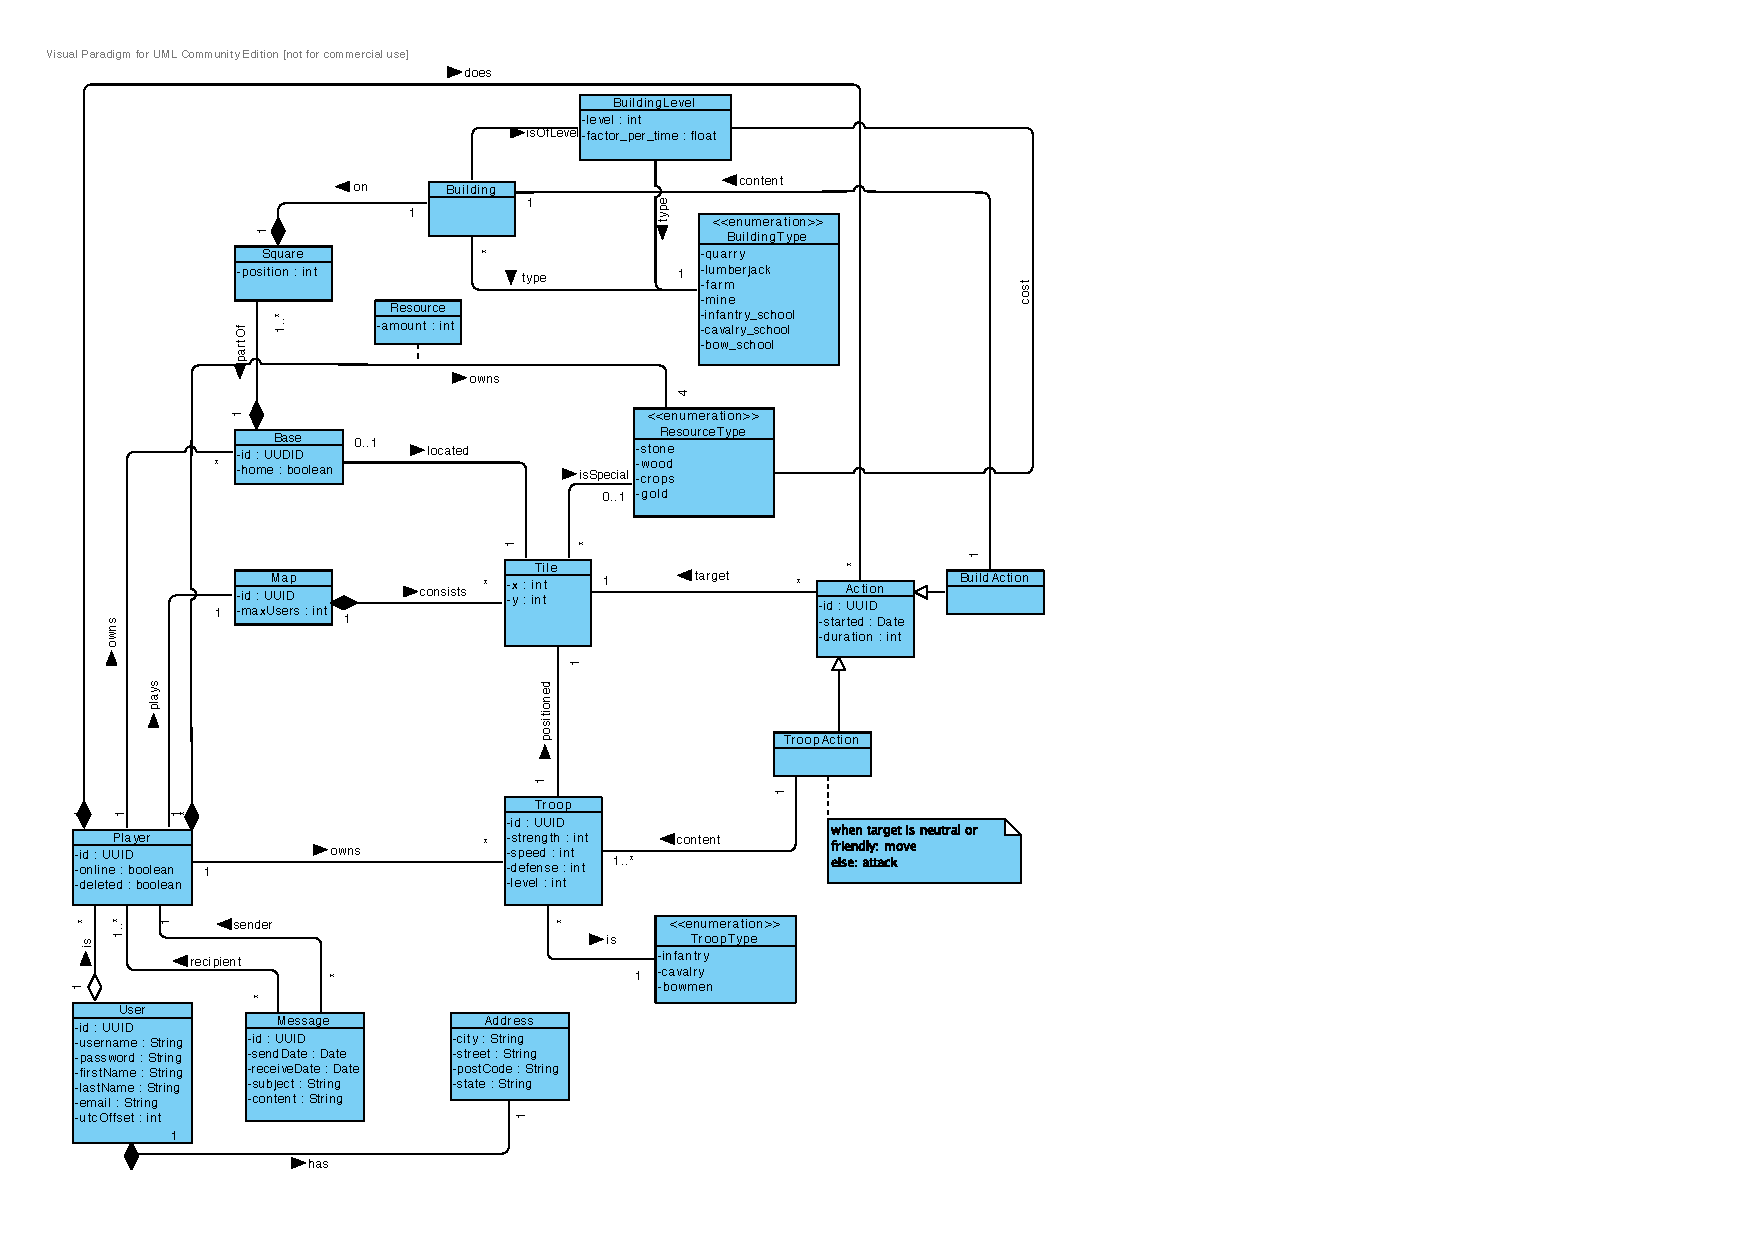
\includegraphics[scale=0.9]{diagrams/SWAG_Class_Diagram.pdf}
\caption{SWAG - Class Diagram}
\label{fig:class}
\end{figure}

\begin{figure}[h]
\center
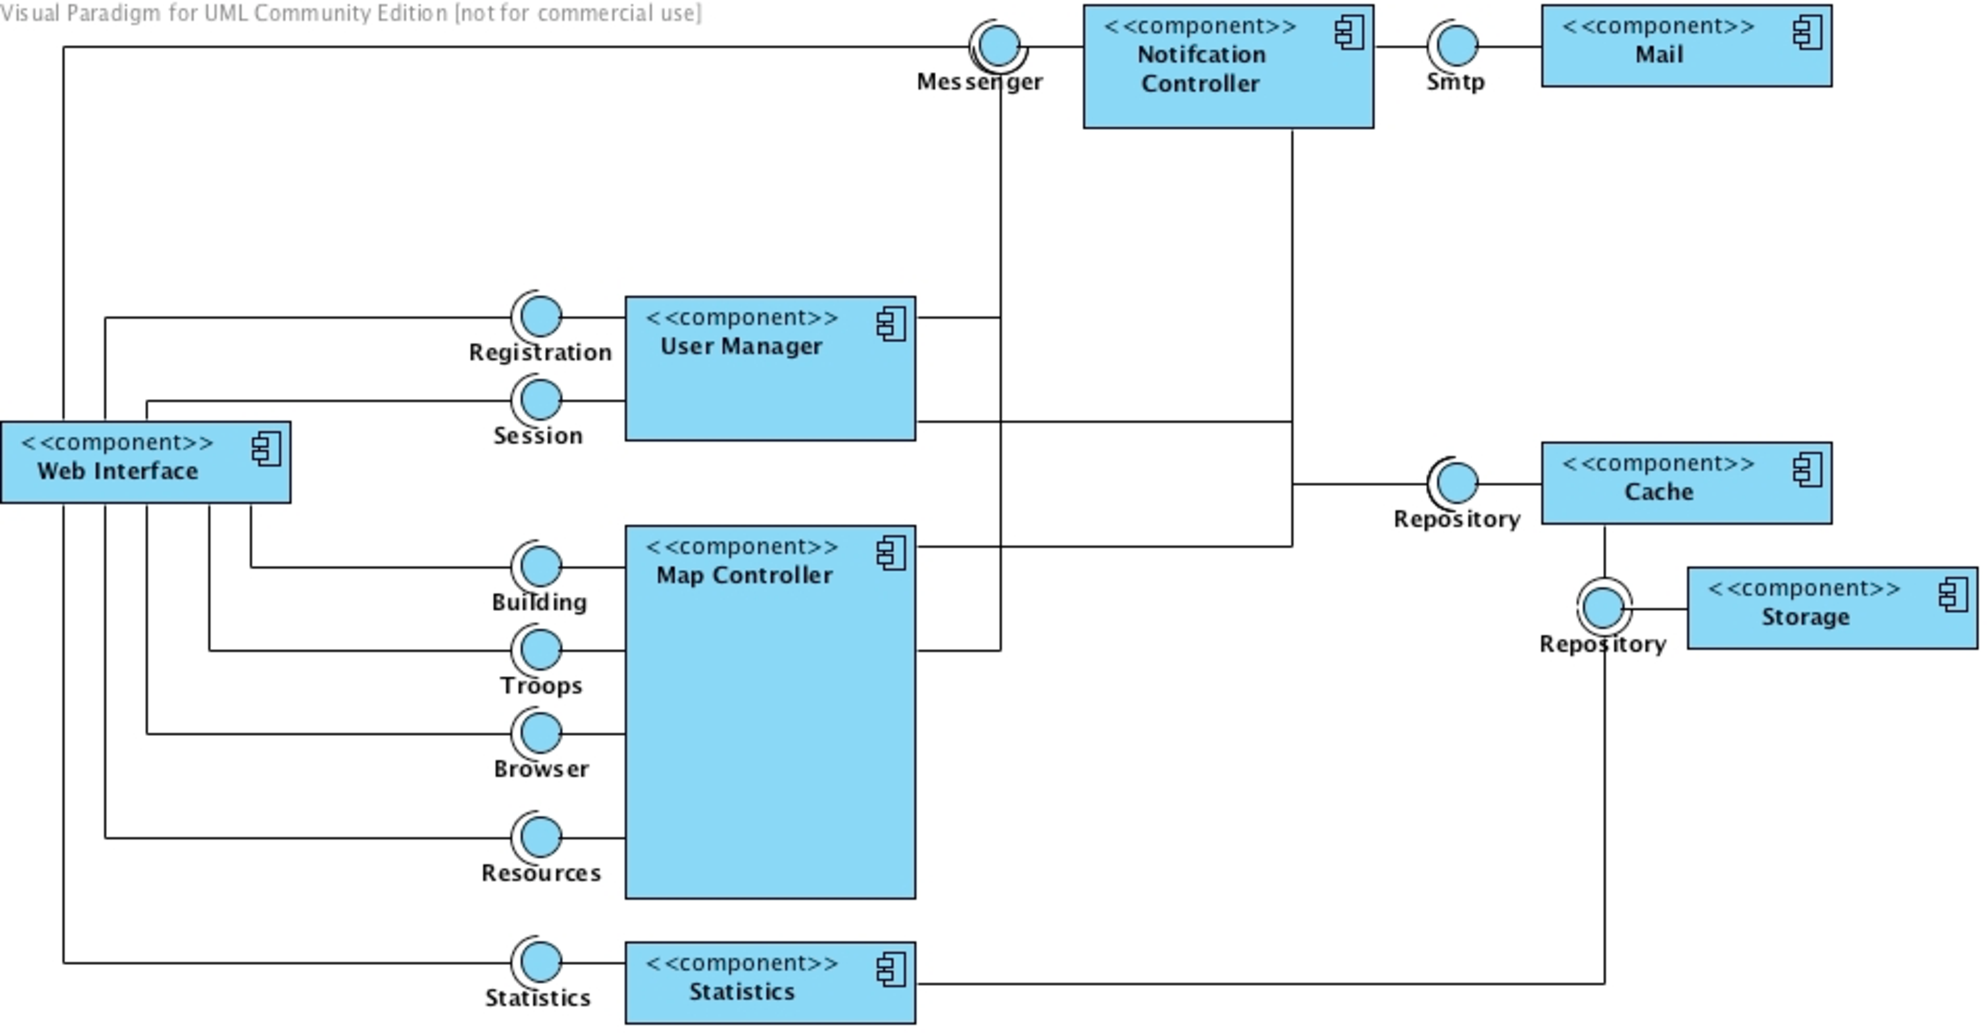
\includegraphics[scale=0.5]{diagrams/SWAG_Component_Diagram.pdf}
\caption{SWAG - Component Diagram}
\label{fig:component}
\end{figure}

\begin{figure}[h]
\hspace{-2cm}
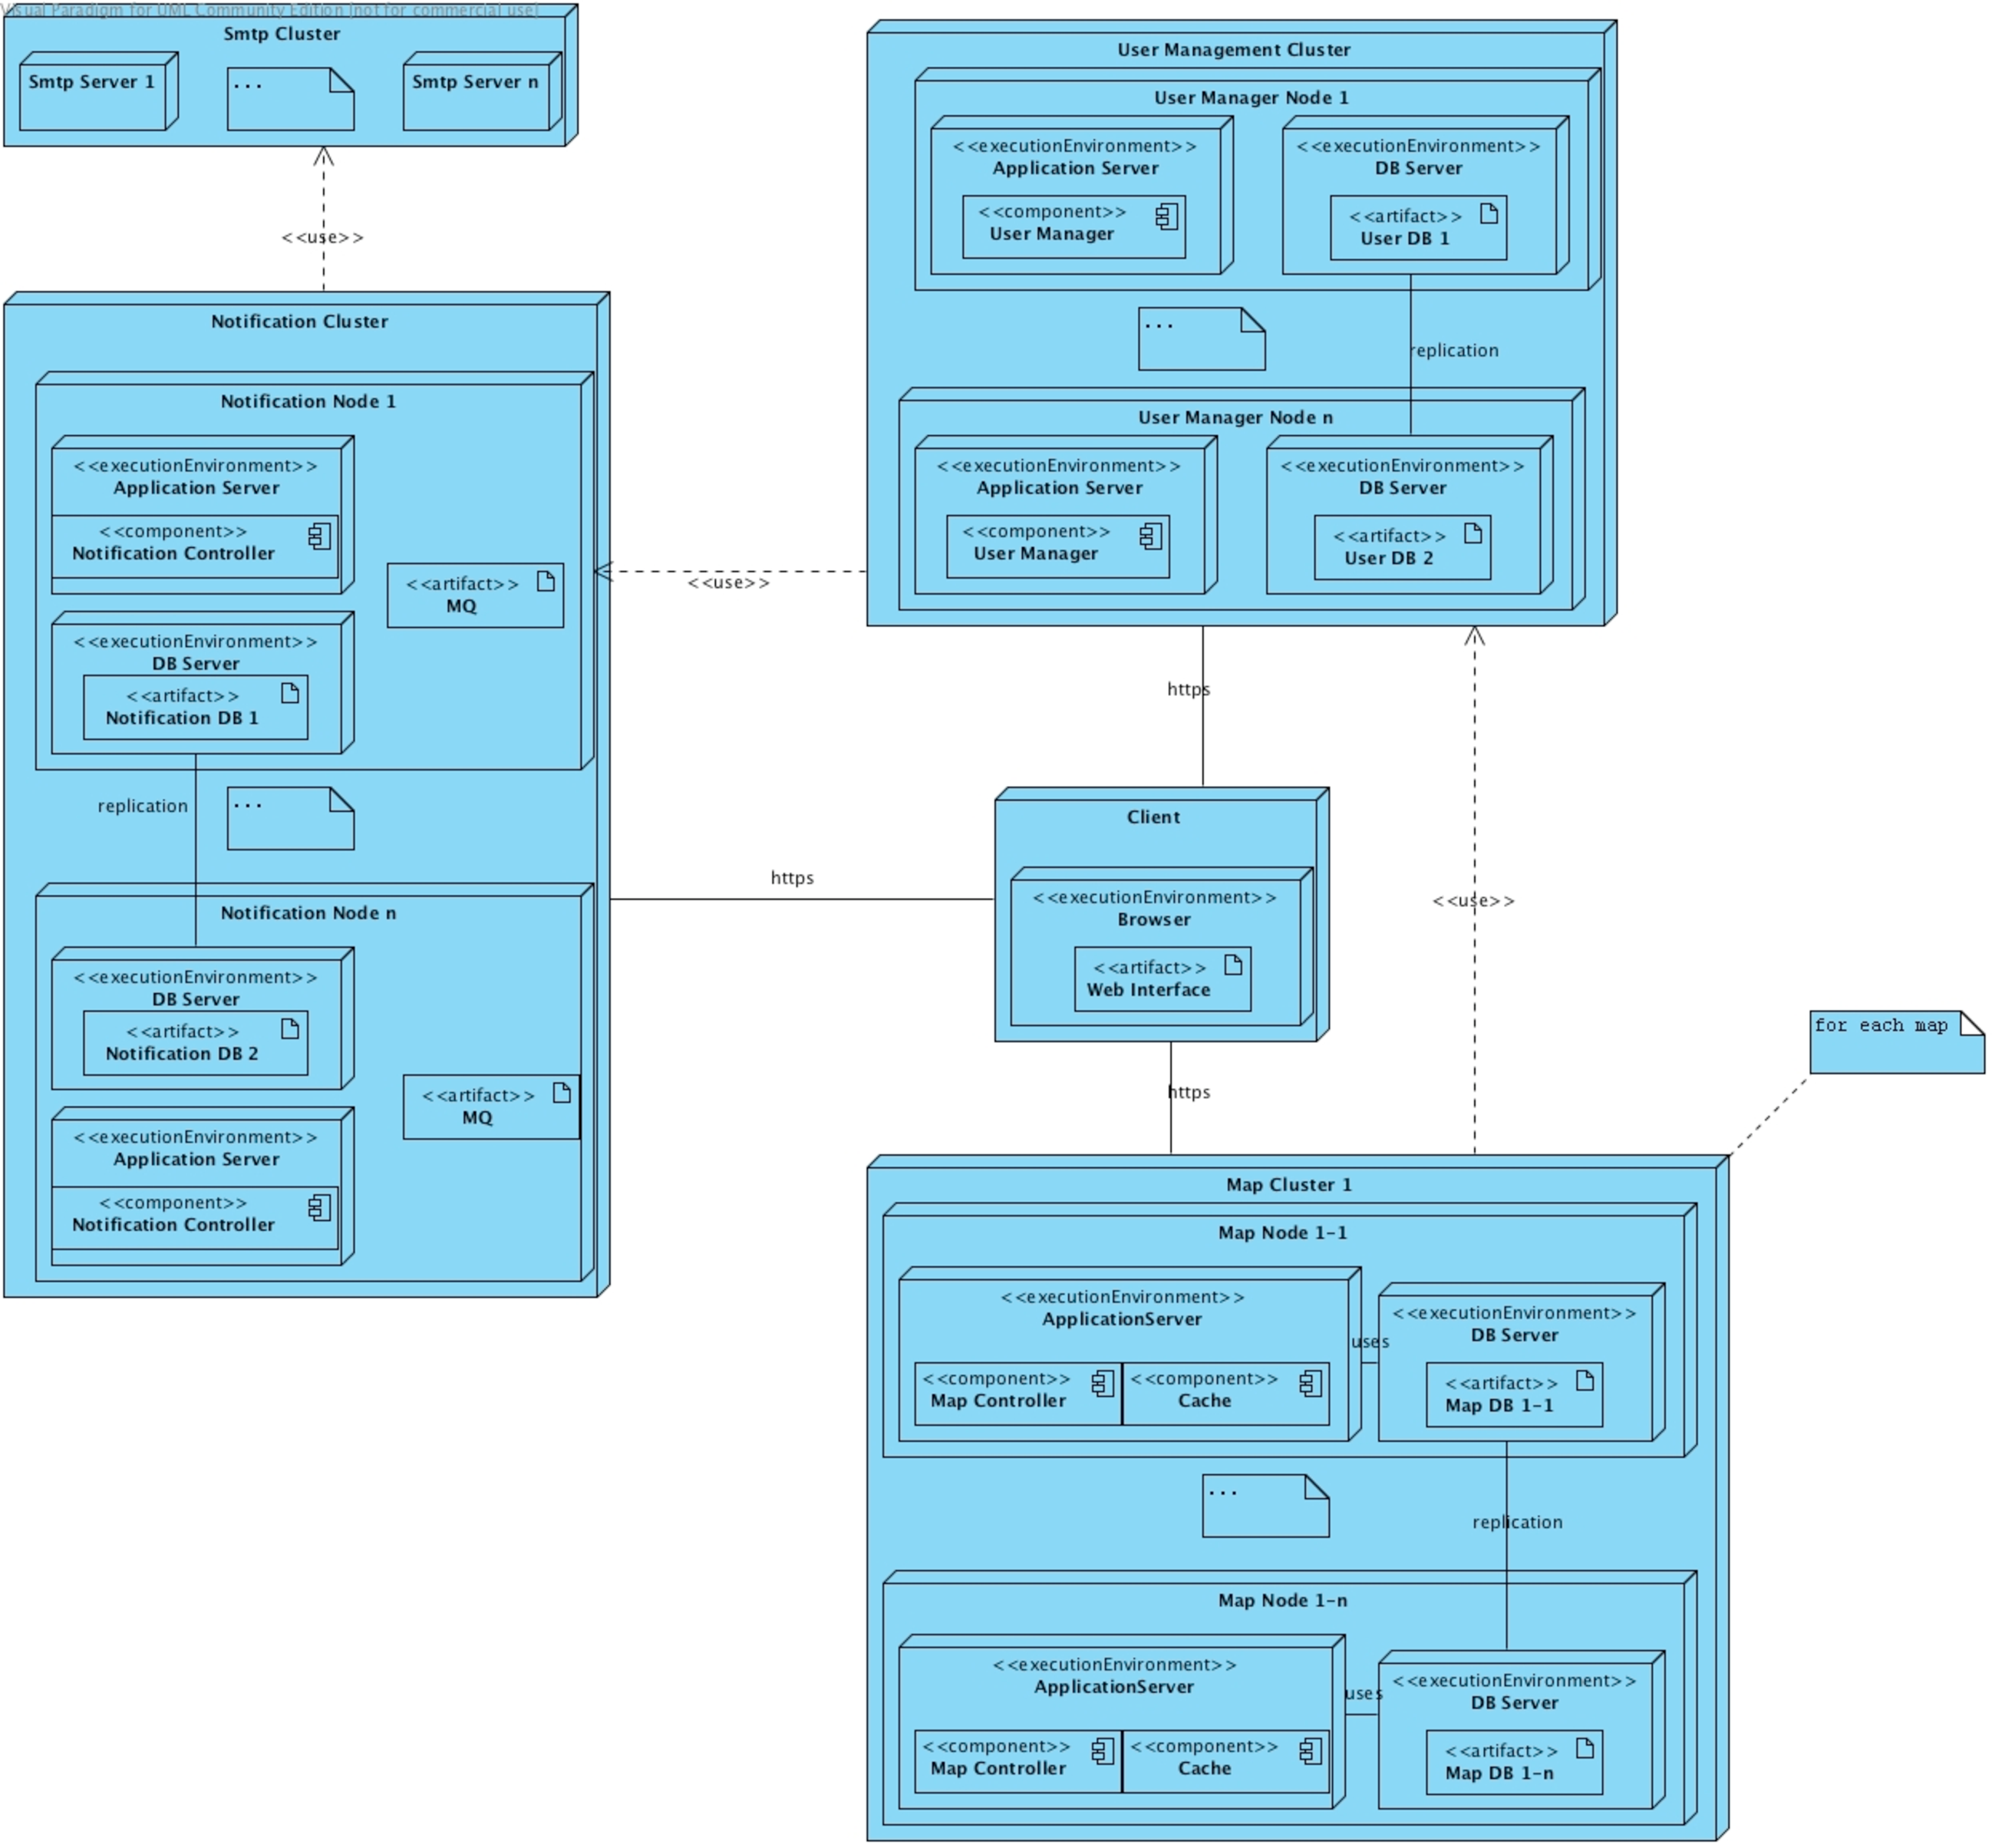
\includegraphics[scale=0.55]{diagrams/SWAG_Deployment_Diagram.pdf}
\caption{SWAG - Deployment Diagram}
\label{fig:deployment}
\end{figure}

 \end{document}

